\chapter{Estado del Arte}\label{chapter:state-of-the-art}

\section{Interfaz de Usuario}

Los tiempos en que solo los científicos y los desarrolladores de \textit{software} podían usar los ordenadores han quedado muy atrás. Hoy en día, casi todo el mundo puede manejar un PC o una tableta, a menudo incluso sin necesitar conocimientos especializados previos. Esto fue posible gracias al desarrollo de las interfaces gráficas de usuario, un tipo de interfaz de usuario.

\subsection{Orígenes}

Las interfaces de usuario existen desde el surgimiento de las computadoras, incluso mucho antes de que se estableciera el campo de la interacción humano-computadora. A lo largo de los años, han aparecido algunos artículos sobre la historia de la interacción humano-computadora y las interfaces de usuario, centrándose principalmente en la era de la interfaz gráfica y los primeros visionarios como Bush, Engelbart y Kay [\cite{5}][\cite{6}][\cite{7}][\cite{8}].

En las primeras computadoras, la interfaz de usuario consistía en la entrada de una tarjeta perforada o un medio equivalente y, aparte de esta consola operativa, los humanos no tenían interacción con estas primeras computadoras en tiempo real.

Las interfaces de usuario complicadas se consideraron un gasto innecesario porque el \textit{software} fue diseñado para utilizar el procesador al máximo. Esto comenzó a cambiar cuando se introdujeron las interfaces de línea de comandos, las cuales redujeron en gran medida la latencia a segundos en lugar de días u horas porque la interfaz de usuario era una serie de transacciones de solicitud y respuesta que permitía al usuario cambiar de opinión sobre las transacciones en respuesta a datos en tiempo real de transacciones anteriores.

La siguiente progresión clave de la interfaz de usuario fue la introducción de terminales de visualización de video. Hacer que sus entradas de comando aparecieran en una pantalla y poder modificarlas de manera inversa fue mucho más rápido que tenerlas impresas. También tenía sentido desde el punto de vista económico al eliminar la necesidad de tinta y materiales de impresión.

%Finalmente, llegó la GUI, originada principalmente en el Centro de Investigación de Palo Alto (PARC) de Xerox, adoptada y mejorada por Apple y estandarizada efectivamente por Microsoft en sus sistemas operativos Windows.

Luego, en los años 70, los primeros conceptos de interfaz gráfica de usuario se desarrollaron en la empresa Xerox. Su propósito principal era permitir manejar ordenadores con el ratón y el teclado en lugar de solo con instrucciones en formato de texto. Xerox Alto fue el primer PC con una interfaz gráfica.

Posteriormente, la llegada de los primeros productos Apple y Microsoft trajo consigo un importante salto adelante en esta materia, tanto así que hoy en día es impensable la interacción con un sistema informático sin este tipo de herramientas virtuales (o naturales) a nuestra disposición.

\subsection{Concepto y características}

La \textbf{interfaz de usuario} (UI por sus siglas en inglés) es el espacio donde se producen las interacciones entre seres humanos y máquinas. El objetivo de esta interacción es permitir el funcionamiento y control más efectivo de la máquina desde la interacción con el humano [\cite{}].

La interfaz de usuario se crea en capas de interacción que apelan a los sentidos humanos (vista, tacto, audición y más). Incluyen tanto dispositivos de entrada como teclado, mouse, micrófono, pantalla táctil, escáner de huellas dactilares y cámara, como dispositivos de salida como monitores, parlantes e impresoras. Los dispositivos que interactúan con múltiples sentidos se denominan ``interfaces de usuario multimedia''. Por ejemplo, la interfaz de usuario cotidiana usa una combinación de entrada táctil (teclado y mouse) y una salida visual y auditiva (monitor y parlantes).

Las interfaces de usuario abarcan tres niveles diferentes de interacción entre humano y máquina, que son:

\begin{itemize}
\item Interfaces de hardware: se refieren únicamente a los componentes físicos y electrónicos del sistema que permiten al usuario introducir y extraer información al sistema. Tal es el caso de teclados, ratones (mouse), pantallas táctiles y/o visualizadoras, etc.
\item Interfaces de software, se refieren al funcionamiento específico de los programas informáticos y de la información virtual que ``ocurre'' o ``tiene lugar'' dentro del computador. Tal es el caso de las aplicaciones que empleamos a diario en nuestro trabajo con computadores.
\item Interfaces de software-hardware: se dedican a establecer un puente entre máquina y usuario, para ``traducir'' las instrucciones humanas al lenguaje del sistema y permitirle llevarlas a cabo exactamente, y al mismo tiempo ``traducir'' las respuestas del sistema del código binario a un lenguaje reconocible por el usuario.
\end{itemize}

Al mismo tiempo, de acuerdo a su manera de interactuar con el usuario, las interfaces pueden clasificarse en:

\begin{itemize}
\item Interfaces de línea de comando (CLI, por sus siglas en inglés), cuando consisten en secuencias de caracteres alfanuméricos, es decir, texto únicamente. Por ejemplo, el MS-DOS.
\item Interfaces gráficas de usuario (GUI, por sus siglas en inglés), cuando reproducen un entorno visual simulado (virtual) cuya lógica permite la comunicación con el usuario. Por ejemplo, Microsoft Windows.
\item Interfaces naturales de usuario (NUI, por sus siglas en inglés), cuando emplean dinámicas “naturales” del ser humano, como el habla o el tacto (mediante pantallas táctiles) para comunicarse directamente con el usuario. Por ejemplo, los programas de IA de servicio personal (como Siri, de Apple).
\end{itemize}

%Otros tipos de interfaces de usuario pueden incluir:

%\begin{itemize}
%\item Interfaz de usuario basada en formularios: se utiliza para ingresar datos en un programa o aplicación al ofrecer una selección limitada de opciones. Por ejemplo, un menú de configuración en un dispositivo se basa en un formulario.
%\item Interfaz gráfica de usuario: conocida también como \textbf{GUI} (del inglés \textit{graphical user interface}), es un programa informático que actúa de interfaz de usuario, utilizando un conjunto de imágenes y objetos gráficos para representar la información y acciones disponibles en la interfaz. Su principal uso consiste en proporcionar un entorno visual sencillo para permitir la comunicación con el sistema operativo de una máquina o computador.
%\item Interfaz de línea de comando: en inglés, \textit{command-line interface}, \textbf{CLI}, es un tipo de interfaz de usuario de computadora que permite a los usuarios dar instrucciones a algún programa informático o al sistema operativo por medio de una línea de texto simple
%\item Interfaz de usuario basada en menús: una interfaz de usuario que utiliza una lista de opciones para navegar dentro de un programa o sitio web. Por ejemplo, los cajeros automáticos utilizan interfaces de usuario basadas en menús y son fáciles de usar para cualquier persona.
%\item Interfaz de usuario táctil: Interfaz de usuario mediante háptica o táctil. La mayoría de los teléfonos inteligentes, tabletas y cualquier dispositivo que funcione con una pantalla táctil utilizan la entrada háptica.
%\item Interfaz de usuario de voz: interacciones entre humanos y máquinas mediante comandos auditivos. Los ejemplos incluyen dispositivos de asistente virtual, hablar a texto y GPS.
%\end{itemize}

La interfaz de usuario es importante para cumplir con las expectativas del usuario y respaldar la funcionalidad efectiva de su sitio.  En términos de visibilidad, su diseño y precisión tienen una importancia primordial para representar la cantidad exacta de información para el usuario previsto. Cada decisión menor tomada para el diseño de la interfaz de usuario puede contribuir al software tanto positiva como negativamente.

%Una interfaz de usuario bien ejecutada facilita la interacción efectiva entre el usuario y el programa, la aplicación o la máquina a través de imágenes contrastantes, diseño limpio y capacidad de respuesta.

%La interfaz de usuario (UI) juega un papel vital en el software. En términos de visibilidad, su diseño y precisión tienen una importancia primordial para representar la cantidad exacta de información para el usuario previsto. Cada decisión menor tomada para el diseño de la interfaz de usuario puede contribuir al software tanto positiva como negativamente.

Más específicamente, estos son los elementos generales más importantes de una gran interfaz de usuario:

%\subsection{Elementos generales de la interfaz de usuario}

%Estos son los elementos generales más importantes de una gran interfaz de usuario:
\begin{itemize}
\item Arquitectura de la información (IA por sus siglas en inglés): La funcionalidad de un sitio se construye de acuerdo a la IA. Es importante estructurar y organizar el contenido de su sitio web de forma lógica para ayudar a los usuarios a navegar por el sitio con el mínimo esfuerzo. Los componentes de IA incluyen tres tipos principales de estructuras organizativas: jerárquica (nivel de importancia), secuencial (orden lógico de pasos) y matricial (en la que el usuario elige la organización del contenido que ve).
Ejemplo: elementos de navegación (botones, pestañas, iconos), etiquetas (terminología), funciones de búsqueda (barra de búsqueda) y sistemas de organización (categorías).
\item Diseño interactivo (ID por sus siglas en inglés): los elementos de ID tienen como objetivo convertir a los lectores pasivos en participantes activos al presentar instancias de entrada del usuario. Tener en cuenta al usuario al crear la interfaz de usuario ayudará a mejorar la interactividad y la ejecución de comportamientos específicos que satisfagan las necesidades del usuario. Además, las interfaces de usuario interactivas diseñadas de manera eficiente pueden ``aprender'' a anticipar y solucionar cualquier problema que pueda surgir antes de que afecte negativamente la experiencia del usuario.
Ejemplo: funciones para compartir en redes sociales, conmutadores, botones.
\item Diseño visual: no se puede subestimar la importancia del valor estético de su sitio. El diseño efectivo utiliza elementos de color, contraste, fuente, video y fotografía para atraer a los visitantes y facilitarles la lectura y trabajar con el contenido, en lugar de alrededor de él, para crear un flujo de funcionalidad lógico e intuitivo.
Ejemplo: Contraste, color, espacio en blanco, tipografía, optimización móvil.
\end{itemize}

\subsection{UI vs UX}

La experiencia de usuario (UX) es la comunicación a través de interfaces, interacción y experiencia que los usuarios tienen con un productos y servicios de la organización.

A menudo se habla de la interfaz de usuario junto con la experiencia del usuario, que puede incluir la apariencia estética del dispositivo, el tiempo de respuesta y el contenido que se presenta al usuario dentro del contexto de la interfaz de usuario. Ambos términos se incluyen en el concepto de interacción humano-computadora (HCI), que es el campo de estudio que se centra en la creación de tecnología informática y la interacción entre humanos y todas las formas de diseño de tecnología informática.

Las principales diferencias entre UX y UI son:

\begin{itemize}
\item La UX gira en torno al propósito y la funcionalidad del producto, mientras que la UI se centra en la calidad de la interacción del usuario con el producto.
\item La UX involucra componentes como la investigación de mercado y la identificación de las necesidades del usuario, mientras que la UI tiene componentes de diseño más artísticos relacionados con la apariencia de la experiencia del usuario.
\item La UX se enfoca en la gestión general de proyectos desde la ideación hasta el desarrollo y la entrega, mientras que la UI se enfoca más específicamente en el diseño del producto terminado.
\end{itemize}

\subsection{Dise\~no de Interfaz de Usuario}

El diseño de interfaz de usuario o ingeniería de la interfaz es el resultado de definir la forma, función, utilidad, ergonomía, imagen de marca y otros aspectos que afectan a la apariencia externa de las interfaces de usuario en sistemas de todo tipo (computadoras de uso general, sistemas de control, dispositivos de comunicación móviles, software de sistemas, software de aplicaciones, sitios web, etc). El objetivo final del diseño de la interfaz de usuario es hacer que la interacción entre el usuario y el sistema del que es interfaz sea tan simple y eficiente como sea posible, en términos de cumplimiento de los objetivos del usuario.

%El objetivo del diseño de una interfaz es producir una interfaz que sea fácil de usar (explicarse por sí misma), eficiente y agradable para que al operar la máquina dé el resultado deseado.

%En general, el objetivo del diseño de la interfaz de usuario es producir una interfaz de usuario que haga que sea fácil, eficiente y agradable (fácil de usar) para operar una máquina de la manera que produce el resultado deseado (es decir, la máxima usabilidad).

En la literatura científica sobre el tema en cuestión aparecen principios que regulan los aspectos que deben caracterizar la Interfaz de Usuario como resultado, es decir asociada al producto, sistema de objetos interactivos y visuales que permiten la comunicación entre los usuarios con el sistema informático.

Hay ocho características consideradas al hacer un buen diseño de interfaz de usuario:
\begin{enumerate}
\item Estética: Un buen diseño de interfaz debe ser atractivo. Significa que el uso de esa interfaz es agradable. El diseño debe incluir características interesantes y fáciles de usar con el atractivo visual.
\item Claridad: es la característica más importante del diseño de la interfaz de usuario. El objetivo principal del diseño de la interfaz de usuario es permitir que el usuario interactúe con el sistema comunicándose con él. La interfaz debe evitar la ambigüedad al dejar todo claro a través del lenguaje, la fluidez, la jerarquía y las metáforas de los elementos visuales.
\item Concisión: Es fácil hacer que la interfaz quede clara clarificando y etiquetando todo en exceso, pero esto lleva a que la interfaz se hinche, donde hay demasiadas cosas en la pantalla al mismo tiempo. Si hay demasiadas cosas en la pantalla, es difícil encontrar lo que está buscando y, por lo tanto, la interfaz se vuelve tediosa de usar. El verdadero desafío para hacer una gran interfaz es hacerla concisa y clara al mismo tiempo.
\item Consistencia: Las interfaces coherentes permiten a los usuarios desarrollar patrones de uso. Los usuarios aprenderán cómo se ven los diferentes botones e íconos y los reconocerán y se darán cuenta de lo que hacen en diferentes contextos. Un diseño único con consistencia habla de un buen diseño de interfaz de usuario.
\item Eficiencia: Un buen diseño de interfaz de usuario le permite realizar diferentes funciones de la aplicación de software o sitio web más rápido y con menos esfuerzo.
\item Familiaridad: Incluso si una persona utiliza una interfaz por primera vez, ciertos elementos aún pueden ser familiares. Las metáforas de la vida real se pueden utilizar para comunicar el significado.
\item Perdón: A veces, el usuario comete errores al usar el software o el sitio web. Manejar el error es un indicador importante de la calidad del software. Un buen diseño de interfaz debería permitir al usuario restaurar los elementos eliminados, lo que en un momento u otro se puede hacer sin querer. La interfaz indulgente es una que puede salvar a los usuarios de errores costosos.
\item Capacidad de respuesta (\textit{responsive} en inglés): Una buena interfaz no debe sentirse lenta. Esto significa que la interfaz debe proporcionar buenos comentarios al usuario sobre lo que está sucediendo y si la entrada del usuario se está procesando correctamente.
\end{enumerate}

%En la literatura científica sobre el tema en cuestión aparecen principios que regulan los aspectos que deben caracterizar la Interfaz de Usuario como resultado, es decir asociada al producto, sistema de objetos interactivos y visuales que permiten la comunicación entre los usuarios con el sistema informático. Es muy poco frecuente encontrar reglas, sistemas de principios que normen el proceso de diseño de interfaces con un enfoque integrador, sustentado en la ingeniería de software y en el carácter multidisciplinar y complejo que posee el mismo. 

%Estos principios sustentan el proceso de Diseño de Interfaz de Usuario en cualquiera de las diferentes aplicaciones informáticas que se pueden desarrollar, con cualquiera de las metodologías de la ingeniería de software, dado su carácter flexible y generalizador y se expresan en las cualidades del diseño de interfaz:

%\begin{itemize}
%\item Confiabilidad: apego a las metodologías del proceso de desarrollo de software asociadas al tránsito por todas las fases y flujos de trabajo de este proceso para la elaboración de la interfaz de usuario.
%\item Multidimensional: su conceptualización, diseño, implementación y validación requieren de un análisis desde diferentes dimensiones tecnológicas, semiótico-visuales así como otras específicas de acuerdo al objetivo, tipo y contenido del producto que se desarrolla.
%\item Multidisciplinar: requiere de la intervención de equipos multidisciplinares que aporten criterios para el desarrollo del proceso en consonancia con el producto.
%\item Usabilidad: asociada a la facilidad de uso, la misma se garantiza a través del uso de técnicas de navegación, selección de objetos visuales, diseño de legibilidad, ergonomía, uso de la tipografía, formatos de ficheros adecuados y otros elementos que propician comodidad ante la interacción con la interfaz.
%\item Accesibilidad: el nivel en que logra transmitir a través de los objetos de la interfaz las diferentes funciones, opciones, componentes, tareas, datos e información contentiva. La inteligibilidad y capacidad de emitir mensajes que favorezcan la comprensión de los objetos que estructuran las diferentes pantallas.
%\item Consistencia: está dada en la estabilidad y solidez de la aplicación, la ejecución libre de errores y la respuesta ante cambios de configuración y soporte a través de la interfaz de usuario.
%\item Funcionalidad: funcionamiento óptimo de la aplicación tomando como referencia los requisitos establecidos, los resultados a obtener y las tareas a resolver mediante espacio de interacción entre usuario-dispositivo.
%\item Interactividad: se concreta en los recursos que se emplean para la retroalimentación de la comunicación entre los usuarios con otros usuarios y los dispositivos a través de la interfaz, de forma que favorezcan el intercambio de información, la orientación hacia diferentes tareas, la información del estado del usuario, la aplicación y los datos.
%\item Hipermedialidad: se basa en el uso adecuado de los recursos visuales para transmitir y comunicar la información, aplicación de los principios de la percepción de las formas y configuración de los elementos básicos del diseño, tales como el color, forma, tipografía, agrupamiento por semejanza, proximidad y jerarquía, identidad visual, homogeneidad de las pantallas, relación objeto-fondo e icono-función, uso de los recursos multimedia.
%\item Adaptabilidad: se sustenta en la capacidad de la interfaz de adaptarse a diferentes plataformas y entornos de trabajo aprovechando las potencialidades de los recursos tecnológicos sin afectación en su funcionalidad.
%\end{itemize}

\subsection{Proceso de diseño de la interfaz de usuario}
El proceso de análisis y diseño de una interfaz de usuario es iterativo y puede representarse mediante un modelo en espiral. El proceso de análisis y diseño de la interfaz de usuario consta de cuatro actividades marco.

\begin{figure}[h]
\centering
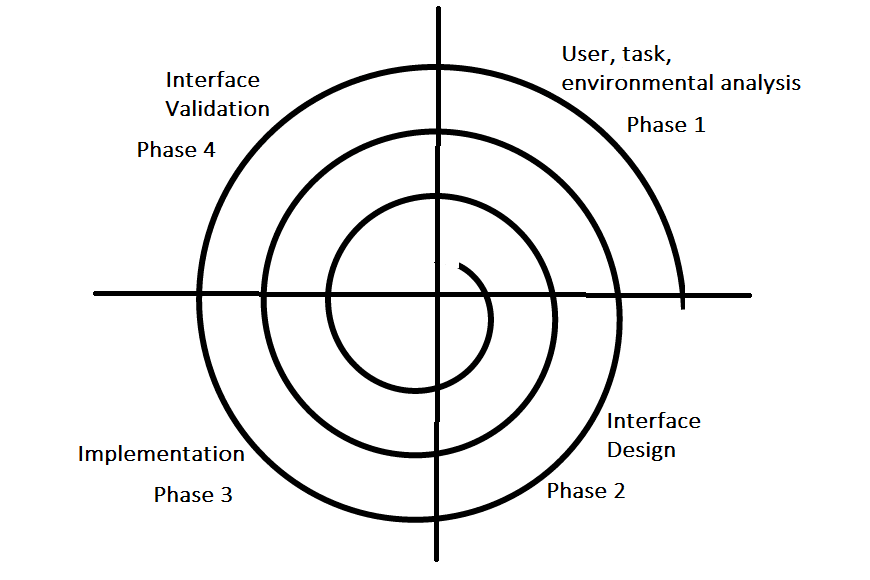
\includegraphics[scale=0.3]{Graphics/espiral}
\caption{Proceso de diseño de interfaz de usuario}
\label{fig:espiral}
\end{figure}

\begin{enumerate}
\item Análisis: El análisis de la interfaz de usuario se centra en el usuario, la tarea, el contenido y el entorno de trabajo que interactúan con el sistema. Inicialmente, el enfoque se basa en el perfil de los usuarios que interactuarán con el sistema, es decir, la comprensión, la habilidad y el conocimiento, el tipo de usuario, etc., según el perfil del usuario, los usuarios se dividen en categorías. De cada categoría se recopilan requisitos. Basado en los requisitos, el desarrollador comprende cómo desarrollar la interfaz. Una vez recopilados todos los requisitos, se realiza un análisis detallado. En la parte de análisis se identifican, describen y elaboran las tareas que realiza el usuario para establecer los objetivos del sistema. El análisis del entorno del usuario se centra en el entorno físico de trabajo.
\item Diseño de la interfaz: el objetivo de esta fase es definir el conjunto de objetos y acciones de la interfaz, es decir, los mecanismos de control que permiten al usuario realizar las tareas deseadas. Indicar cómo estos mecanismos de control afectan al sistema. Especificar la secuencia de acciones de tareas y subtareas, también denominada escenario de usuario. Indicar el estado del sistema cuando el usuario realiza una determinada tarea. Siempre seguir las tres reglas de oro establecidas por Theo Mandel. Los problemas de diseño como el tiempo de respuesta, la estructura de comando y acción, el manejo de errores y las funciones de ayuda se consideran a medida que se refina el modelo de diseño. Esta fase sirve como base para la fase de implementación.
\item Construcción e implementación de la interfaz: La actividad de implementación comienza con la creación de un prototipo (modelo) que permite evaluar escenarios de uso. A medida que continúa el proceso de diseño iterativo, se puede utilizar un conjunto de herramientas de interfaz de usuario que permite la creación de ventanas, menús, interacción de dispositivos, mensajes de error, comandos y muchos otros elementos de un entorno interactivo para completar la construcción de una interfaz.
\item Validación de la interfaz: esta fase se centra en probar la interfaz. La interfaz debería ser tal que debería poder realizar tareas correctamente y debería poder manejar una variedad de tareas. Debe cumplir con todos los requisitos del usuario. Debe ser fácil de usar y fácil de aprender. Los usuarios deben aceptar la interfaz como útil en su trabajo.
\end{enumerate}

Las pruebas determinan la efectividad de una aplicación de interfaz de usuario que debe probarse y expone qué tan fácil o difícil es usar la interfaz de usuario para la audiencia más amplia posible. Los dos principales tipos de pruebas son los siguientes:

\begin{enumerate}
\item Pruebas de usabilidad: evalúan un producto estudiando cómo los usuarios reales realmente usan el sistema. Proporciona una recuperación significativa solo cuando está bien integrado en todo el ciclo de vida del proyecto.
\item Pruebas de accesibilidad: acceden a la aplicación de prueba con tecnologías accesibles y herramientas de prueba automatizadas.
\end{enumerate}

\section*{Usabilidad}


\section*{Accesibilidad}



%El diseño de interacción tiene que ver con la interacción de la visión del usuario y la pantalla, ya sea que sepa qué tocar, deslizar o hacer clic, y si lo que sucede cumple con sus expectativas y lo acerca a sus objetivos. El diseño de interacción se trata de tomar la visualización final de cómo las personas deben usar lo que ha diseñado con ellos y qué beneficios puede brindarles una mejor experiencia para que puedan comprender cómo actuar. Todo el proceso incluido en el diseño de interacción no tiene relación con las fuentes, colores, estilo, etc. El objetivo total es el movimiento de tareas, la disposición secuencial de eventos y la confirmación de que el usuario obtendrá los aspectos visuales que lo dirigirán. ella en esas actividades.

%El diseño de la interfaz se basa completamente en las imágenes, como la apariencia de la interfaz, la disposición de varios elementos y la interconectividad entre ellos en términos de jerarquía. La elección de la selección de fuentes, los esquemas de color, los elementos gráficos, los botones y el El estilo del menú se incluye en el diseño de la interfaz. Los diseñadores de interfaces también pueden poner sus ideas en las cosas que ya están decididas y han estado en el producto durante mucho tiempo, sus ideas se implementarán si se está mejorando la experiencia del usuario.


\section{Vuejs}

\section{Typescript}

\section{Pinia}

\section{Usabilidad}